\documentclass[11pt, letterpaper]{article}
\usepackage[top=1in, bottom=1in, left=1in, right=1in]{geometry}

% Math, graphics, and bibliography
\usepackage{amsmath,amssymb,amsfonts,mathrsfs,mathtools}
\usepackage{graphicx}
\usepackage[round,numbers,sort&compress]{natbib}
\renewcommand{\bibnumfmt}[1]{#1.}

% My preferred fonts
\usepackage[T1]{fontenc}
\usepackage{lmodern}
\usepackage[sc]{mathpazo}

% For fancier fractions and figure captions
\usepackage[labelfont={bf}, margin=1cm]{caption}
\usepackage{units}
\usepackage{booktabs}

% For supplemental figures
\newcommand{\beginsupplement}{%
        \setcounter{table}{0}
        \renewcommand{\thetable}{S\arabic{table}}%
        \setcounter{figure}{0}
        \renewcommand{\thefigure}{S\arabic{figure}}%
     }

% Puts the affiliations on the cover page
\usepackage{authblk}

\begin{document}
\title{Quantifying stochastic noise in cultured\\ circadian reporter cells}
\author[1]{Peter C. St. John}
\author[1,*]{Francis J. Doyle III}
\affil[1]{Department of Chemical Engineering, University of California Santa
Barbara, Santa Barbara, California 93106-5080}
\affil[*]{Email: \texttt{doyle@engineering.ucsb.edu}}
\date{\today}
\maketitle

\begin{center}
Running head:\\ {Quantifying circadian stochastic noise} \\[1ex]
Keywords:\\ Systems Biology | Circadian Rhythms \\ Gene
Regulatory Network | Stochastic | Synchronization
\end{center}

\pagebreak
\begin{abstract}

\end{abstract}

\section*{Introduction}

Circadian rhythms in mammals are daily changes in physiology and gene expression that persist even in the absence of external environmental cues.


\section*{Materials and Methods}

\section*{Results and Discussion}

\begin{figure}[tbp]
  \begin{center}
    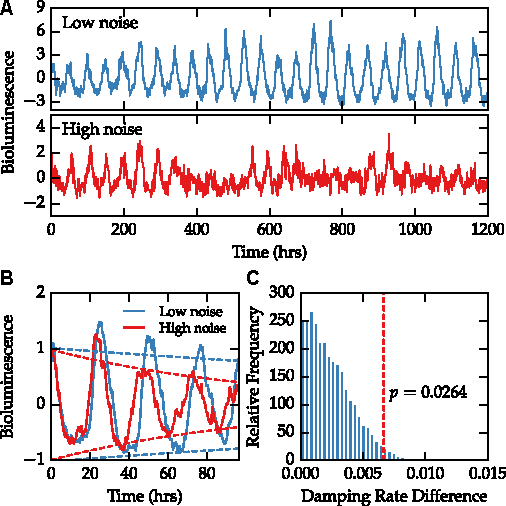
\includegraphics[]{figures/pdfs/noise_ts_and_boot.pdf}
  \end{center}
  \caption{{\bfseries Figure Title.}
({\bfseries A}) Part A.
({\bfseries B}) Part B.
({\bfseries C}) Part C.}
\label{fig:fibroblast_noise}
\end{figure}


\begin{figure}[tbp]
  \begin{center}
    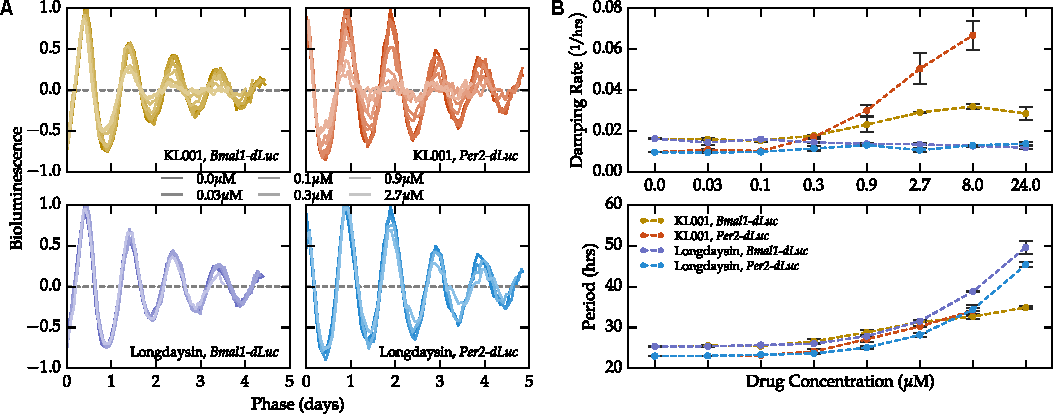
\includegraphics[]{figures/pdfs/mainfig_dose.pdf}
  \end{center}
  \caption{{\bfseries Figure Title.}
({\bfseries A}) Part A.
({\bfseries B}) Part B.}
\label{fig:dose_dependence}
\end{figure}


\begin{figure}[tbp]
  \begin{center}
    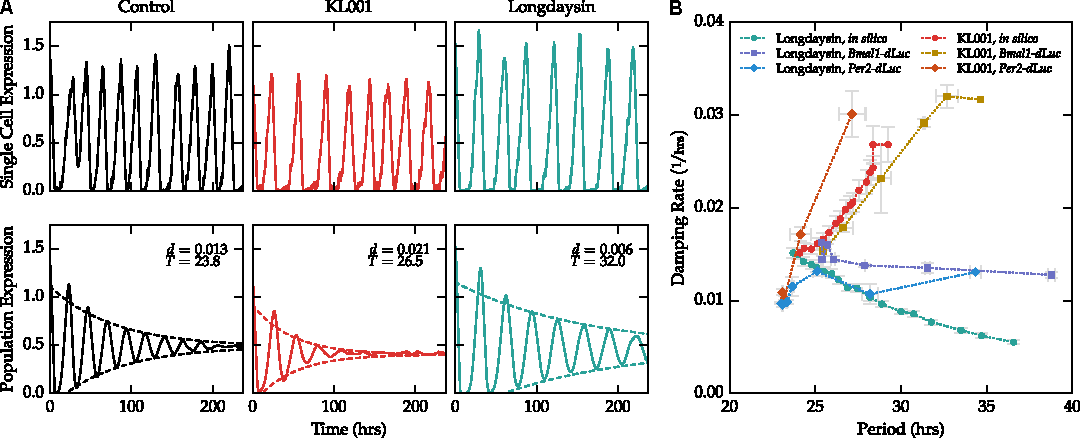
\includegraphics[]{figures/pdfs/main_fig_simulations.pdf}
  \end{center}
  \caption{{\bfseries Figure Title.}
({\bfseries A}) Part A.
({\bfseries B}) Part B.}
\label{fig:simulation}
\end{figure}


\begin{figure}[tbp]
  \begin{center}
    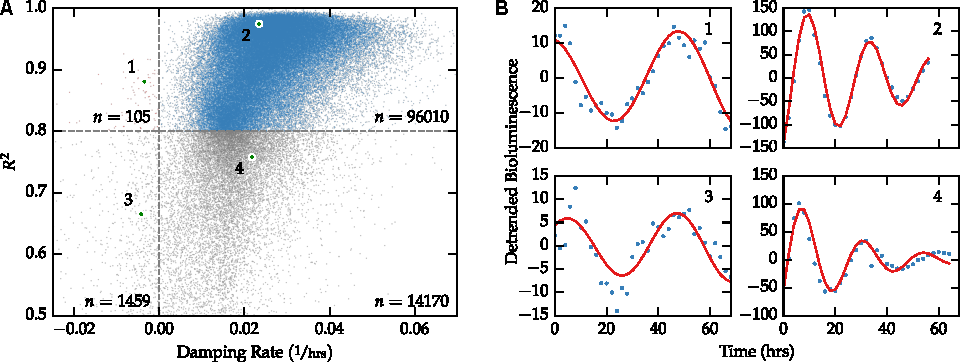
\includegraphics[]{figures/pdfs/r2_vs_decay.pdf}
  \end{center}
  \caption{{\bfseries Figure Title.}
({\bfseries A}) Part A.
({\bfseries B}) Part B.}
\label{fig:fit_quality}
\end{figure}


\begin{figure}[tbp]
  \begin{center}
    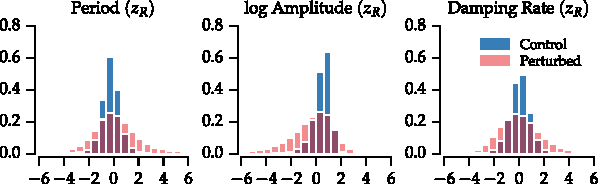
\includegraphics[]{figures/pdfs/fitted_parameters.pdf}
  \end{center}
  \caption{{\bfseries Figure Title.}
({\bfseries A}) Part A.
({\bfseries B}) Part B.}
\label{fig:fit_distributions}
\end{figure}


\begin{table}
  \begin{center}
    \begin{tabular}{lrrrrrr}\toprule
      {} & \multicolumn{2}{c}{$T$} & \multicolumn{2}{c}{$\ln A$} & \multicolumn{2}{c}{$d$} \\
      {}         & \multicolumn{1}{c}{C}         & \multicolumn{1}{c}{P}           & \multicolumn{1}{c}{C}         & \multicolumn{1}{c}{P}               & \multicolumn{1}{c}{C}         & \multicolumn{1}{c}{P}           \\\midrule
      $\mu$      & $-0.234$  & $0.187$  &  $0.443$  & $-0.343$  &  $0.043$  & $0.090$    \\
      $\sigma$   & $ 0.774$  & $1.820$  &  $0.778$  & $ 1.753$  &  $0.878$  & $1.688$    \\
      Skew & $ 0.153$  & $0.367$  & -$1.823$  & $-0.580$  & -$0.107$  & $0.371$    \\
      Kurt & $ 3.772$  & $0.591$  &  $8.329$  & $ 0.476$  &  $2.423$  & $0.373$    \\
      \bottomrule
    \end{tabular}
  \end{center}
  \caption{{\bfseries Fitted Parameters}}
  \label{tab:fit_distributions}
\end{table}


\begin{table}
  \begin{center}
    \begin{tabular}{rrrrr}
      \toprule
      {}       & $d$    & $\ln A$ & $T$    & $\theta$ \\\midrule
      $d$      & $1.000 $ & $0.285 $  & $-0.142$ & $-0.269$\\\
      $\ln A$  & $0.285 $ & $1.000 $  & $-0.022$ & $-0.112$\\
      $T$      & $-0.142$ & $-0.022$  & $1.000 $ & $-0.113$\\
      $\theta$ & $-0.269$ & $-0.112$  & $-0.113$ & $1.000 $\\
      \bottomrule
    \end{tabular}
  \end{center}
  \caption{{\bfseries Correlation matrix}}
  \label{tab:corr}
\end{table}


\begin{figure}[tbp]
  \begin{center}
    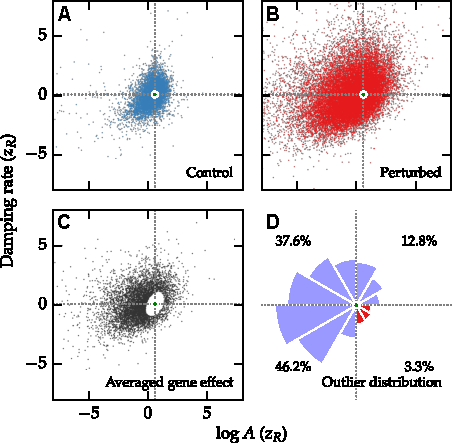
\includegraphics[]{figures/pdfs/outliers.pdf}
  \end{center}
  \caption{{\bfseries Figure Title.}
({\bfseries A}) Part A.
({\bfseries B}) Part B.}
\label{fig:outlier_dist}
\end{figure}




\section*{Conclusion}

\section*{Acknowledgments}
This work was supported by the National Institutes of Health/National Institute of General Medical Sciences under award number 1R01GM096873-01 and by the Institute for Collaborative Biotechnologies through grant W911NF-09-0001 from the U.S.\ Army Research Office.


% \bibliographystyle{biophysj.bst}
% \bibliography{condensed_library.bib}

\beginsupplement

\begin{figure}[tbp]
  \begin{center}
    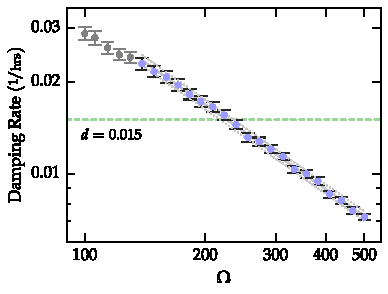
\includegraphics[]{figures/pdfs/volume_calibration.pdf}
  \end{center}
  \caption{{\bfseries Figure Title.}
({\bfseries A}) Part A.
({\bfseries B}) Part B.}
\label{fig:vol_calibration}
\end{figure}

\begin{figure}[tbp]
  \begin{center}
    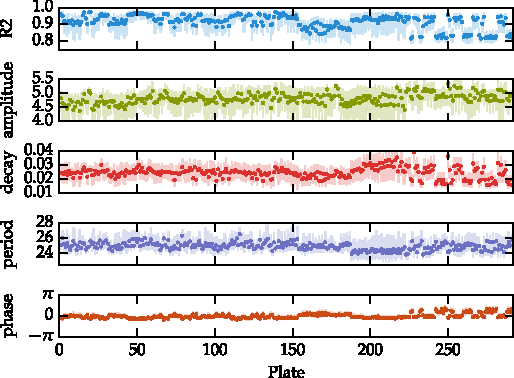
\includegraphics[]{figures/pdfs/zhang_plates.pdf}
  \end{center}
  \caption{{\bfseries figure title.}
({\bfseries a}) part a.
({\bfseries b}) part b.}
\label{fig:plate_variation}
\end{figure}

\begin{figure}[tbp]
  \begin{center}
    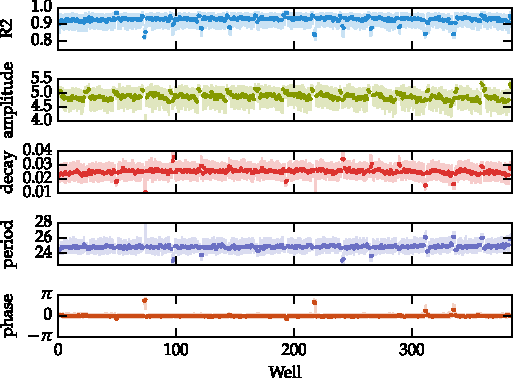
\includegraphics[]{figures/pdfs/zhang_wells.pdf}
  \end{center}
  \caption{{\bfseries figure title.}
({\bfseries a}) part a.
({\bfseries b}) part b.}
\label{fig:well_variation}
\end{figure}

\begin{table}
\begin{center}
\begin{tabular}{lclc}
\toprule
\textbf{Dep. Variable:}    &      decay       & \textbf{  R-squared:         } &$     0.169  $\\
\textbf{Model:}            &       OLS        & \textbf{  Adj. R-squared:    } &$     0.169  $\\
\textbf{Method:}           &  Least Squares   & \textbf{  F-statistic:       } &$     4782.  $\\
\textbf{Date:}             & Wed, 11 Feb 2015 & \textbf{  Prob (F-statistic):} &$     0.00   $\\
\textbf{Time:}             &     16:26:22     & \textbf{  Log-Likelihood:    } &$-1.7248e+05 $\\
\textbf{No. Observations:} &       94053      & \textbf{  AIC:               } &$ 3.450e+05  $\\
\textbf{Df Residuals:}     &       94048      & \textbf{  BIC:               } &$ 3.450e+05  $\\
\bottomrule
\end{tabular}
\begin{tabular}{lccccc}
                   & \textbf{coef} & \textbf{std err} & \textbf{t} & \textbf{P$>$$|$t$|$} & \textbf{[95.0\% Conf. Int.]}  \\
\midrule
\textbf{const}     &     $-0.0370$ &       $0.014$    &   $-2.572$ &        $0.010$       &       $-0.065,  -0.009$      \\
\textbf{amplitude} &     $ 0.2375$ &       $0.003$    &   $86.282$ &        $0.000$       &       $ 0.232,   0.243$      \\
\textbf{period}    &     $-0.1521$ &       $0.003$    &   $56.798$ &        $0.000$       &       $-0.157,  -0.147$      \\
\textbf{phase}     &     $-0.2354$ &       $0.003$    &   $85.598$ &        $0.000$       &       $-0.241,  -0.230$      \\
\textbf{type}      &     $ 0.3197$ &       $0.015$    &   $20.664$ &        $0.000$       &       $ 0.289,   0.350$      \\
\bottomrule
\end{tabular}
\begin{tabular}{lclc}
\textbf{Omnibus:}       &$9769.391$& \textbf{  Durbin-Watson:     } &$    1.876$ \\
\textbf{Prob(Omnibus):} &$  0.000 $& \textbf{  Jarque-Bera (JB):  } &$18459.719$ \\
\textbf{Skew:}          &$  0.697 $& \textbf{  Prob(JB):          } &$     0.00$ \\
\textbf{Kurtosis:}      &$  4.664 $& \textbf{  Cond. No.          } &$     8.34$ \\
\bottomrule
\end{tabular}
\end{center} 
\caption{OLS Regression Results}
\label{tab:ols_reg}
\end{table}


\end{document}

